\section{\textbf{Descrição do sistema}}
\label{descricao-do-sistema}

% Antes de descrever qualquer coisa relacionada a ferramenta, é preciso entender que o \textit{software} passa por um aprendizado de máquina para aprender os padrões de características que são necessária para atender as necessidades do projeto, que é reconhecer um jogador em campo. O \textit{haar cascade} fica responsável por realizar a classificação da imagem para obter seus padrões de características. Basicamente, o \textit{haar cascade} é alimentado manualmente por imagens aleatórias de jogadores para montar um padrão de características e em seguida, esses padrões são treinados através do \textit{machine learning}. Isso deve ser feito para que seja possível obter um modelo de busca. Pode-se definir o modelo de busca como padrão de características de jogadores de futebol americano que será utilizado para realizar a busca.

O \textit{software} apresentado no decorrer deste projeto tem por objetivo reconhecer um jogador dentro de campo utilizando as técnicas de processamento de imagem para realizar a extração de todas as características importantes que estão presentes em uma imagem.

Antes de descrever qualquer coisa relacionada à ferramenta, é preciso entender que o \textit{software} passa por um aprendizado de máquina para extrair os padrões de características que são necessária para atender as necessidades do projeto, que é reconhecer um jogador em campo. Portanto, o sistema conta com a classificação de imagem para extrair as características relacionadas aos jogadores de futebol americano, conforme representado na \autoref{fig_ext_caracteristicas}.

\begin{figure}[h]
	\caption{\label{fig_ext_caracteristicas}Etapa de extração de características de uma imagem (A) e seu padrão de características (B).}
	\begin{center}
		\resizebox{.9\linewidth}{!}{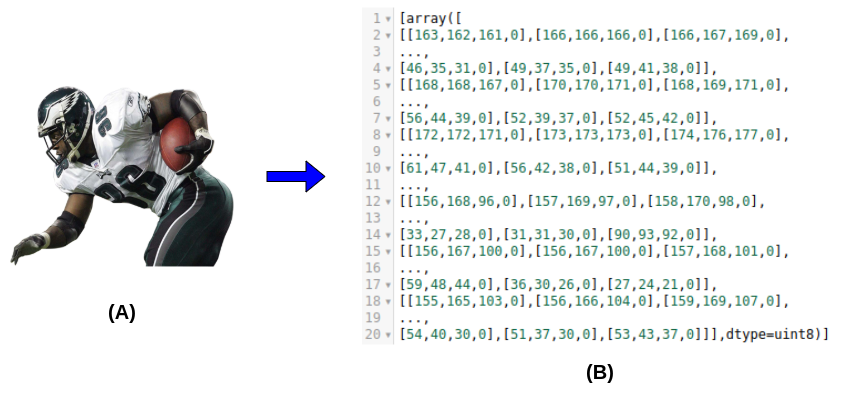
\includegraphics{6-Desenvolvimento-Projeto/imagens-desenvolvimento/conversao-de-imagem.png}}
	\end{center}
	\centering \legend{Fonte: Elaborada pelos autores.}
\end{figure}

% O \textit{haar cascade} fica responsável por realizar a classificação da imagem para obter seus padrões de características. Basicamente, o mesmo é alimentado manualmente por imagens aleatórias de jogadores de futebol americano para montar esse padrão de características. Sendo assim, pode-se definir o modelo de busca como o conjunto de padrões de características de jogadores de futebol americano que será utilizado para realizar a busca.

Quem fica responsável por realizar a classificação das imagens para obter seus padrões de características é o \textit{haar cascade}. Basicamente, o mesmo é alimentado manualmente por imagens aleatórias de jogadores de futebol americano para montar esse padrão de características. Sendo assim, pode-se definir o modelo de busca como um conjunto de padrões de características de jogadores de futebol americano que será utilizado para realizar a busca.

Em seguida, o \textit{software} passa pela etapa de \textit{machine learning} que ficará encarregada apenas de treinar o algoritmo utilizando os padrões de características. Ou seja, nessa etapa do processo, o sistema recebe como parâmetro os padrões de características extraídos na etapa anterior e analisa todos os seus pontos de interesse, montando o melhor modelo de busca.

Em seguida, o sistema recebe, através do dispositivo de captura de imagem, um vídeo em tempo real de uma partida de futebol americano.

O algoritmo realiza a análise de todos os \textit{frames}\footnote{\textit{Frames} por segundo é a taxa de atualização de imagens estáticas que formam uma cena animada dentro de um vídeo. A ilusão que nosso cérebro interpreta como movimento é feita através de vários quadros consecutivos em um curto período de tempo \cite{FRAMES2011}. \label{frames-por-segundo}} por segundo do vídeo para encontrar algo similar ao modelo de busca que foi treinado.

Caso ocorra a identificação de um jogador de futebol americano dentro do vídeo analisado, o algoritmo fica encarregado de realizar uma representação do mesmo. Essa representação será feita com um contorno verde ao redor do jogador.